\documentclass{article}
\usepackage{amsmath}
\usepackage{amsthm}
\usepackage{amssymb}
\usepackage{tikz}
\usepackage{braket}

\newtheorem*{polarizador*}{Definición}
\newtheorem*{vars*}{Definición}
\newtheorem*{inter*}{Definición}

\begin{document}
\section*{Básicos}
La \textbf{mecánica cuántica} es actualmente la mejor forma que tenemos de describir los fenómenos más fundamentales. En sí misma, esta es una \textbf{herramienta de trabajo}, aplicada a diferentes campos:
\begin{itemize}
    \item \textbf{Electrodinámica cuántica}: mecánica cuántica aplicada a electromagnetismo.
    \item \textbf{Óptica cuántica}: mecánica cuántica aplicada a los fotones.
\end{itemize}
\pagebreak
\section*{Linealidad}
A la hora de trabajar con una teoría que describa como funciona nuestro mundo, tenemos una serie de \textbf{variables dinámicas}  (variables no constantes) cuyo valor queremos conocer ya que están relacionadas con la observación de estos fenómenos. Los valores obtenidos en los cálculos de un experimento se pueden comparar a los valores observados durante la ejecución de dicho experimento.\\

\noindent\fbox{%
    \parbox{\textwidth}{%
    Un ejemplo de una \textbf{teoría lineal} es la \textbf{teoría del electromagnetismo de Maxwell}. Esto quiere decir que podemos sumar directamente las soluciones de dos fenómenos diferentes para obtener como funcionan en su conjunto, sin cambiar nada.
    Por ejemplo, con el campo generado \textbf{indivudalmente}  por dos cargas $q_{1}$ y $q_{2}$, podemos saber como funcionan en su conjunto si sumamos ambos campos: $\vec{E_{T}}=\vec{E_{1}}+\vec{E_{2}}$.
    }%
}
\pagebreak
\section*{Ecuación lineal}
Una ecuación linear es la que tiene la siguiente forma:
\[
    L(u)=0
\]
Donde $L$ es un operador lineal y $u$ es cualquier valor. Para que $L$ sea un operador lineal, debe cumplir las siguientes propiedades:
\begin{itemize}
    \item $L(k \cdot u)=k\cdot L(u)$
    \item $L(u_1+u_2)=L(u_1)+L(u_2)$
\end{itemize}
\subsection*{Ejemplo}
Sea una ecuación lineal la siguiente:
\[
    \frac{du}{dt}+ \frac{1}{\tau}u=0
\]
Podemos definir $Lu$ como:
\[
    Lu=0
\]
tal que:
\[
    Lu=\frac{du}{dt}+ \frac{1}{\tau}u
\]
Si quisiéramos obtener el operador $L$ por individual, tendríamos:
\[
    L= \frac{d}{dt} +\frac{1}{\tau}
\]
Vamos a comprobar si $L$ es \textbf{lineal}:
\begin{itemize}
    \item $L ku =\frac{dku}{dt} + \frac{1}{\tau}ku= k(\frac{du}{dt}+ \frac{1}{\tau}u)$ \checkmark
    \item $L(u+v)=\frac{d(u+v)}{dt}+ \frac{1}{\tau}(u+v)=\frac{du}{dt}+ \frac{1}{\tau}u+\frac{dv}{dt}+ \frac{1}{\tau}v\:$ \checkmark
\end{itemize}
\pagebreak
\section*{Mecánica cuántica}
La mecánica cuántica \textbf{es lineal}, y la ecuación que describe su movimiento 
es la \textbf{ecuación de Schrödinger}. La \textbf{variable dinámica}  de esta ecuación 
es la \textbf{función de onda} $(\Psi)$. Esta función de onda depende de $t$ (tiempo). Esta ecuación es:
\[
    i\hbar \frac{\partial\Psi}{\partial t}=\hat{H}\Psi
\]
Donde $\hat{H}$ es el \textbf{Hamiltoniano}, un operador lineal.
Si definimos esta ecuación como $L \Psi=0$, obtenemos que:
\[
    L \Psi =i\hbar \frac{\partial\Psi}{\partial t}- \hat{H}\Psi
\]
Se puede observar que $L$ en este caso es un \textbf{operador lineal}, lo que implica que esta ecuación \textbf{es una ecuación lineal}.
\pagebreak
\section*{Necesidad de números complejos}
En la ecuación de Schrödinger, aparece el valor $i$, definido como:
\[
    i=\sqrt{-1}
\]
Un número complejo $z$ se define como:
\[
    z=a+bi\mid \in \mathbb{C}
\]
\begin{itemize}
    \item $Re(z)=a\mid a\in \mathbb{R}$: parte \textbf{real}.
    \item $Im(z)= b \mid b \in \mathbb{R}$: parte \textbf{imaginaria}.
\end{itemize}
Definimos el \textbf{conjugador} de $z$ como $z^{*}$ siendo este:
\[
    z^{*}=a-bi
\]
La \textbf{norma} (o módulo) de un número complejo se define como:
\[
    |z|=\sqrt{a^{2}+b^{2}}\mid |z|\in \mathbb{R}
\]
tal que:
\[
    |z|^2=a^2+b^2=zz^{*}
\]
Como un número complejo se puede representar en un plano de dos dimensiones $(x,y)$, podemos representar este número complejo mediante su \textbf{ángulo} $(\theta)$ respecto de la línea de los reales:
\[
    z=\cos \theta + i \sin \theta=e^{i \theta}
\]
Por tanto:
\[
    \Psi \in \mathbb{C}
\]
Esto implica dos hechos importantes:
\begin{itemize}
    \item \textbf{Todas las soluciones son imaginarias}: puesto que $\Psi$ es imaginario por definición, todas las soluciones \textbf{serán imaginarias}.
    \item \textbf{No se pueden medir números imaginarios}
\end{itemize}
Esto conlleva al problema de que, si la ecuación de onda es imaginaria, ¿cual es su interpretación física?\\
La ``solución'' a este problema fue deducida por \textbf{Max Born}. Este físico y matemático interpretó que la \textbf{norma} de la función de onda era una \textbf{probabilidad}:
\[
    |\Psi|^{2} \propto p
\]
\noindent\fbox{%
    \parbox{\textwidth}{%
    El famoso gato de Schrödinger fue una analogía para ejemplificar la ridiculez de esta teoría basada en probabilidades.
    }%
}
\pagebreak
\section*{Determinismo}
Tras el trabajo de Einstein, Planck, Maxwell, etc, se observó que los fotones tenían comportamientos tanto de \textbf{onda}  como de \textbf{partícula}. Einstein descubrió que la energía de un fotón era:
\[
    E=h f
\]
Donde $f$ es la frecuencia de la luz, tal que:
\[
    \lambda f =c
\]

\subsection*{Un polarizador}
\begin{polarizador*}[Polarizador]
    Material que deja pasar la luz o 
no en función de si esta está alineada con su dirección de preferencia. En 
la imagen, la dirección de preferencia es la flecha, que está alineada con el 
\textbf{eje X}. La luz alineada con este eje \textbf{pasará completamente}. Por
 el contrario, la luz alineada con el eje Y, \textbf{no pasará}.
\end{polarizador*}
\tikzset{every picture/.style={line width=0.75pt}} %set default line width to 0.75pt        



\tikzset{every picture/.style={line width=0.75pt}} %set default line width to 0.75pt        

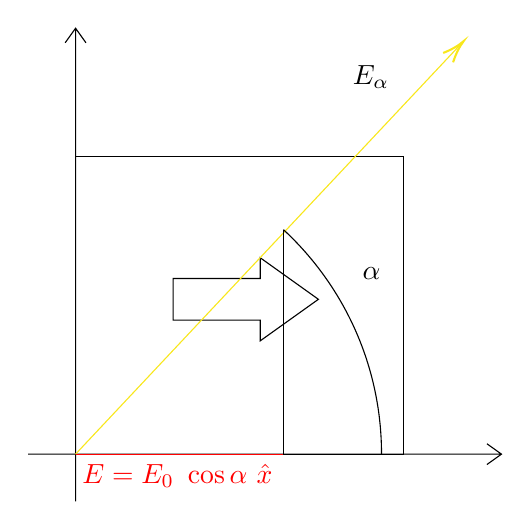
\begin{tikzpicture}[x=0.75pt,y=0.75pt,yscale=-1,xscale=1]
%uncomment if require: \path (0,300); %set diagram left start at 0, and has height of 300

%Shape: Rectangle [id:dp8316254942548869] 
\draw   (193,106.4) -- (351,106.4) -- (351,249.6) -- (193,249.6) -- cycle ;
%Right Arrow [id:dp04340175452480244] 
\draw   (240,165) -- (282,165) -- (282,155) -- (310,175) -- (282,195) -- (282,185) -- (240,185) -- cycle ;
%Shape: Axis 2D [id:dp1403743813430538] 
\draw  (170.2,249.6) -- (398.2,249.6)(193,44.4) -- (193,272.4) (391.2,244.6) -- (398.2,249.6) -- (391.2,254.6) (188,51.4) -- (193,44.4) -- (198,51.4)  ;
%Straight Lines [id:da29159927135813013] 
\draw [color={rgb, 255:red, 248; green, 231; blue, 28 }  ,draw opacity=1 ]   (193,249.6) -- (378.63,52.06) ;
\draw [shift={(380,50.6)}, rotate = 133.22] [color={rgb, 255:red, 248; green, 231; blue, 28 }  ,draw opacity=1 ][line width=0.75]    (10.93,-3.29) .. controls (6.95,-1.4) and (3.31,-0.3) .. (0,0) .. controls (3.31,0.3) and (6.95,1.4) .. (10.93,3.29)   ;
%Shape: Arc [id:dp47095655248343604] 
\draw  [draw opacity=0] (293.16,141.44) .. controls (322.29,168.44) and (340.43,207.01) .. (340.41,249.6) -- (193,249.6) -- cycle ; \draw   (293.16,141.44) .. controls (322.29,168.44) and (340.43,207.01) .. (340.41,249.6) ;  
%Straight Lines [id:da8079360725677336] 
\draw    (293.16,249.6) -- (293.16,141.44) ;
%Straight Lines [id:da97570509264987] 
\draw [color={rgb, 255:red, 255; green, 1; blue, 1 }  ,draw opacity=1 ]   (193,249.6) -- (293.16,249.6) ;

% Text Node
\draw (330,158.4) node [anchor=north west][inner sep=0.75pt]    {$\alpha $};
% Text Node
\draw (195,253) node [anchor=north west][inner sep=0.75pt]    {$\textcolor[rgb]{1,0,0}{E=E_{0} \ \cos \alpha \ \hat{x}}$};
% Text Node
\draw (325.4,61.1) node [anchor=north west][inner sep=0.75pt]    {$E_{\alpha }$};


\end{tikzpicture}


\[
    \vec{E_\alpha}=E_0 \cos \alpha \hat{x} + E_0 \sin \alpha \hat{y}
\]
Tras pasar por el \textbf{polarizador}:
\[
    E=E_0 \cos \alpha \hat{x}
\]
La fracción de fotones que pasa es:
\[
    \frac{|E|}{|E_a|}=\frac{E_0^2\cos^2 \alpha}{E_0^2}=\cos^2 \alpha  
\]
Sin embargo, esto es ciertamente incorrecto, ya que no pueden pasar una fracción de fotones. O bien pasan todos, o bien no pasan ninguno. En física clásica, lo que le pasa a un fotón, le pasa a todos.
En la experimentación, observamos que llevando a cabo el mismo experimento, \textbf{obtenemos diferentes resultados}. A veces pasan los fotones, y a veces no.\\
En conclusión, \textbf{se ha perdido el determinismo}.

\section*{Variables ocultas}
Tras el desastre que supuso la apartente pérdida del determinismo, Einstein, junto a otros, trataron de explicar que la razón por la que apararentemente
era imposible predecir el comportamiento de los fotones era debido a la existencia de \textbf{variables ocultas}.
\begin{vars*}[Variables ocultas]
    Variables o características de un sistema que determinan el comportamiento de este, pero que sin embargo son desconocidas para el observador,
    y que por tanto podrían explicar la razón por la que no podemos predecir estos comportamientos. En sí, la naturaleza de estos permite predecirlos,
    pero carecemos de la información necesaria para hacerlo.
\end{vars*}

\section*{Representar fotones}
Para representar los movimientos de fotones como vectores, Paul Dirac inventó una notación para representarlos utilizando als funciones de onda. Si
queremos representar un \textbf{fotón} moviendóse en el eje $\mathrm{X}$, se representaría de la siguiente forma:
\[
     \ket{\text{fotón}; x}
\]
o en el eje $\mathrm{Y}$:
\[
    \ket{\text{fotón}; y}
\]
Gracias a la linealidad, si queremos representar estos dos estados como una única \textbf{superposición}, simplemente debemos sumarlos y multiplicarlos
por su respectiva razón trigonométrica. El estado de este fotón se representaría así:
\[
    \ket{\text{fotón}; \alpha}= \cos \alpha \ket{\text{fotón}; x}+\sin \ket{\text{fotón}; y}
\]
\pagebreak

\section*{Superposición}
Para ilustrar la naturaleza de la superposición cuántica, una de las herramientas que allanarán el camino será el \textbf{interferómetro Mach-Zehnder}.
\begin{inter*}[Interferómetro]
    Dispositivo que utiliza las interferencias de ondas para medir longitudes de onda, velocidades de onda y otras características.
\end{inter*}
Este dispositivo tiene un \textbf{divisor de haz} como se muestra en el siguiente diagrama:



\tikzset{every picture/.style={line width=0.75pt}} %set default line width to 0.75pt        

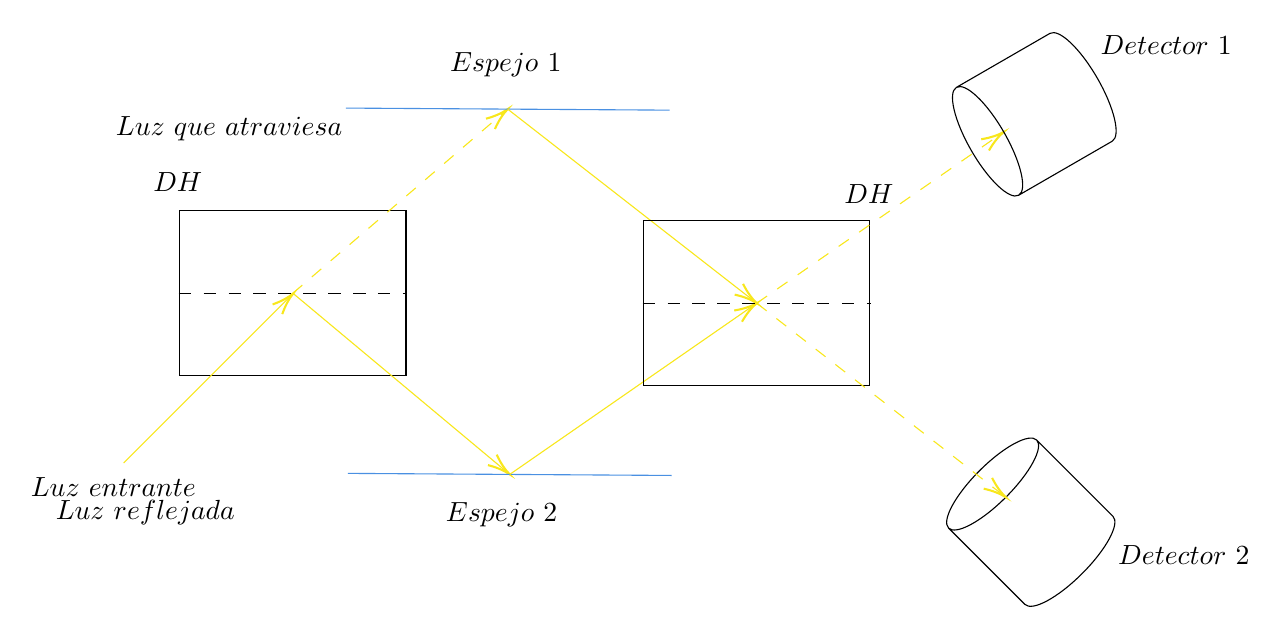
\begin{tikzpicture}[x=0.75pt,y=0.75pt,yscale=-1,xscale=1]
%uncomment if require: \path (0,300); %set diagram left start at 0, and has height of 300

%Shape: Rectangle [id:dp11037996736515354] 
\draw   (128,103) -- (237,103) -- (237,182.6) -- (128,182.6) -- cycle ;
%Straight Lines [id:da24241112155752842] 
\draw  [dash pattern={on 4.5pt off 4.5pt}]  (127.5,142.8) -- (237.5,142.8) ;
%Straight Lines [id:da582785337201249] 
\draw [color={rgb, 255:red, 248; green, 231; blue, 28 }  ,draw opacity=1 ]   (101,224.6) -- (181.39,144.21) ;
\draw [shift={(182.8,142.8)}, rotate = 135] [color={rgb, 255:red, 248; green, 231; blue, 28 }  ,draw opacity=1 ][line width=0.75]    (10.93,-3.29) .. controls (6.95,-1.4) and (3.31,-0.3) .. (0,0) .. controls (3.31,0.3) and (6.95,1.4) .. (10.93,3.29)   ;
%Straight Lines [id:da7010071953198695] 
\draw [color={rgb, 255:red, 248; green, 231; blue, 28 }  ,draw opacity=1 ]   (182.5,142.8) -- (285.47,228.82) ;
\draw [shift={(287,230.1)}, rotate = 219.88] [color={rgb, 255:red, 248; green, 231; blue, 28 }  ,draw opacity=1 ][line width=0.75]    (10.93,-3.29) .. controls (6.95,-1.4) and (3.31,-0.3) .. (0,0) .. controls (3.31,0.3) and (6.95,1.4) .. (10.93,3.29)   ;
%Straight Lines [id:da6331889030186113] 
\draw [color={rgb, 255:red, 248; green, 231; blue, 28 }  ,draw opacity=1 ] [dash pattern={on 4.5pt off 4.5pt}]  (182.5,142.8) -- (284.48,55.4) ;
\draw [shift={(286,54.1)}, rotate = 139.4] [color={rgb, 255:red, 248; green, 231; blue, 28 }  ,draw opacity=1 ][line width=0.75]    (10.93,-3.29) .. controls (6.95,-1.4) and (3.31,-0.3) .. (0,0) .. controls (3.31,0.3) and (6.95,1.4) .. (10.93,3.29)   ;
%Straight Lines [id:da4384360838133676] 
\draw [color={rgb, 255:red, 74; green, 144; blue, 226 }  ,draw opacity=1 ]   (209,229.6) -- (365,230.6) ;
%Straight Lines [id:da06667761792048621] 
\draw [color={rgb, 255:red, 74; green, 144; blue, 226 }  ,draw opacity=1 ]   (208,53.6) -- (364,54.6) ;
%Straight Lines [id:da023069454494369923] 
\draw [color={rgb, 255:red, 248; green, 231; blue, 28 }  ,draw opacity=1 ]   (287,230.1) -- (404.36,148.74) ;
\draw [shift={(406,147.6)}, rotate = 145.27] [color={rgb, 255:red, 248; green, 231; blue, 28 }  ,draw opacity=1 ][line width=0.75]    (10.93,-3.29) .. controls (6.95,-1.4) and (3.31,-0.3) .. (0,0) .. controls (3.31,0.3) and (6.95,1.4) .. (10.93,3.29)   ;
%Straight Lines [id:da6543160810720763] 
\draw [color={rgb, 255:red, 248; green, 231; blue, 28 }  ,draw opacity=1 ]   (286,54.1) -- (404.42,146.37) ;
\draw [shift={(406,147.6)}, rotate = 217.92] [color={rgb, 255:red, 248; green, 231; blue, 28 }  ,draw opacity=1 ][line width=0.75]    (10.93,-3.29) .. controls (6.95,-1.4) and (3.31,-0.3) .. (0,0) .. controls (3.31,0.3) and (6.95,1.4) .. (10.93,3.29)   ;
%Shape: Rectangle [id:dp6923714844204956] 
\draw   (351.5,107.8) -- (460.5,107.8) -- (460.5,187.4) -- (351.5,187.4) -- cycle ;
%Straight Lines [id:da9366936816953415] 
\draw  [dash pattern={on 4.5pt off 4.5pt}]  (351,147.6) -- (461,147.6) ;
%Shape: Can [id:dp2637359566131918] 
\draw   (540.85,213.52) -- (577.62,250.29) .. controls (581.13,253.81) and (574.49,266.15) .. (562.77,277.87) .. controls (551.05,289.59) and (538.71,296.23) .. (535.19,292.72) -- (498.42,255.95) .. controls (494.91,252.43) and (501.56,240.09) .. (513.27,228.37) .. controls (524.99,216.66) and (537.33,210.01) .. (540.85,213.52) .. controls (544.36,217.04) and (537.72,229.38) .. (526,241.1) .. controls (514.28,252.82) and (501.94,259.46) .. (498.42,255.95) ;
%Straight Lines [id:da4719418003068032] 
\draw [color={rgb, 255:red, 248; green, 231; blue, 28 }  ,draw opacity=1 ] [dash pattern={on 4.5pt off 4.5pt}]  (406,147.6) -- (524.42,239.87) ;
\draw [shift={(526,241.1)}, rotate = 217.92] [color={rgb, 255:red, 248; green, 231; blue, 28 }  ,draw opacity=1 ][line width=0.75]    (10.93,-3.29) .. controls (6.95,-1.4) and (3.31,-0.3) .. (0,0) .. controls (3.31,0.3) and (6.95,1.4) .. (10.93,3.29)   ;
%Straight Lines [id:da8897684247143063] 
\draw [color={rgb, 255:red, 248; green, 231; blue, 28 }  ,draw opacity=1 ] [dash pattern={on 4.5pt off 4.5pt}]  (406,147.6) -- (523.36,66.24) ;
\draw [shift={(525,65.1)}, rotate = 145.27] [color={rgb, 255:red, 248; green, 231; blue, 28 }  ,draw opacity=1 ][line width=0.75]    (10.93,-3.29) .. controls (6.95,-1.4) and (3.31,-0.3) .. (0,0) .. controls (3.31,0.3) and (6.95,1.4) .. (10.93,3.29)   ;
%Shape: Can [id:dp21598285016890628] 
\draw   (502.21,43.62) -- (547.24,17.62) .. controls (551.54,15.13) and (561.75,24.75) .. (570.03,39.1) .. controls (578.32,53.45) and (581.54,67.1) .. (577.24,69.58) -- (532.21,95.58) .. controls (527.9,98.07) and (517.7,88.45) .. (509.41,74.1) .. controls (501.13,59.75) and (497.9,46.1) .. (502.21,43.62) .. controls (506.51,41.13) and (516.72,50.75) .. (525,65.1) .. controls (533.28,79.45) and (536.51,93.1) .. (532.21,95.58) ;

% Text Node
\draw (122,131) node [anchor=north west][inner sep=0.75pt]   [align=left] {};
% Text Node
\draw (55,230.4) node [anchor=north west][inner sep=0.75pt]    {$Luz\ entrante$};
% Text Node
\draw (67,241.4) node [anchor=north west][inner sep=0.75pt]    {$Luz\ reflejada$};
% Text Node
\draw (96,56.4) node [anchor=north west][inner sep=0.75pt]    {$Luz\ que\ atraviesa$};
% Text Node
\draw (257,25.4) node [anchor=north west][inner sep=0.75pt]    {$Espejo\ 1$};
% Text Node
\draw (255,242.4) node [anchor=north west][inner sep=0.75pt]    {$Espejo\ 2$};
% Text Node
\draw (114,83.4) node [anchor=north west][inner sep=0.75pt]    {$DH$};
% Text Node
\draw (447,89.4) node [anchor=north west][inner sep=0.75pt]    {$DH$};
% Text Node
\draw (570.4,17.6) node [anchor=north west][inner sep=0.75pt]    {$Detector\ 1$};
% Text Node
\draw (578.9,263.1) node [anchor=north west][inner sep=0.75pt]    {$Detector\ 2$};


\end{tikzpicture}

Ahora bien, este experimento debería plantearse como que cada haz de luz representa fotones individuales. Debido a que este experimento trabaja con interferencias,
es importante definir qué son estas interferencias.\\
Si por un lado tenermos interferencias \textbf{destructivas}, es intuitivo pensar que dos fotones se \textbf{destruyen}, entre sí. Sin embargo, esto es
imposible, ya que violaría la \textbf{ley de conservación de energía}. De la misma forma, si interfiriésen de forma constructiva, no se obtendrían más fotones
ni más energía.\\
Lo que en realidad está pasando, es que cada haz de luz es una \textbf{posible posición} del fotón, todas superpuestas, y las interferencias son
estas \textbf{superposiciones} cancelándose y aumentándose entre sí.\\
Al pasar por el primer divisor, el fotón está en los dos haces de luz a la vez, y cuando llega al segundo, el fotón interfiere consigo mismo, donde
se determina su posición final.

\subsection*{Estados y vectores}
Cuando hablamos de estados, podemos asociar estos con vectores. Sin embargo, un único vector puede ser representado como la \textbf{suma} de otros vectores:


\tikzset{every picture/.style={line width=0.75pt}} %set default line width to 0.75pt        

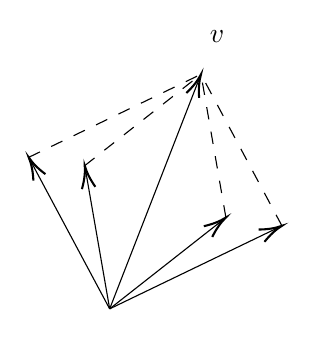
\begin{tikzpicture}[x=0.75pt,y=0.75pt,yscale=-1,xscale=1]
%uncomment if require: \path (0,300); %set diagram left start at 0, and has height of 300

%Straight Lines [id:da4374883380605319] 
\draw    (213,203.6) -- (201.34,136.57) ;
\draw [shift={(201,134.6)}, rotate = 80.13] [color={rgb, 255:red, 0; green, 0; blue, 0 }  ][line width=0.75]    (10.93,-3.29) .. controls (6.95,-1.4) and (3.31,-0.3) .. (0,0) .. controls (3.31,0.3) and (6.95,1.4) .. (10.93,3.29)   ;
%Straight Lines [id:da009103297012910128] 
\draw    (213,203.6) -- (267.43,160.84) ;
\draw [shift={(269,159.6)}, rotate = 141.84] [color={rgb, 255:red, 0; green, 0; blue, 0 }  ][line width=0.75]    (10.93,-3.29) .. controls (6.95,-1.4) and (3.31,-0.3) .. (0,0) .. controls (3.31,0.3) and (6.95,1.4) .. (10.93,3.29)   ;
%Straight Lines [id:da22204878180178] 
\draw  [dash pattern={on 4.5pt off 4.5pt}]  (201,134.6) -- (257,90.6) ;
%Straight Lines [id:da29223223295901235] 
\draw  [dash pattern={on 4.5pt off 4.5pt}]  (269,159.6) -- (257,90.6) ;
%Straight Lines [id:da8103478172957961] 
\draw    (213,203.6) -- (256.27,92.46) ;
\draw [shift={(257,90.6)}, rotate = 111.27] [color={rgb, 255:red, 0; green, 0; blue, 0 }  ][line width=0.75]    (10.93,-3.29) .. controls (6.95,-1.4) and (3.31,-0.3) .. (0,0) .. controls (3.31,0.3) and (6.95,1.4) .. (10.93,3.29)   ;
%Straight Lines [id:da947641501103899] 
\draw    (213,203.6) -- (174.94,132.36) ;
\draw [shift={(174,130.6)}, rotate = 61.89] [color={rgb, 255:red, 0; green, 0; blue, 0 }  ][line width=0.75]    (10.93,-3.29) .. controls (6.95,-1.4) and (3.31,-0.3) .. (0,0) .. controls (3.31,0.3) and (6.95,1.4) .. (10.93,3.29)   ;
%Straight Lines [id:da18315811974555407] 
\draw  [dash pattern={on 4.5pt off 4.5pt}]  (174,130.6) -- (257,90.6) ;
%Straight Lines [id:da29550623174968105] 
\draw    (213,203.6) -- (294.2,164.47) ;
\draw [shift={(296,163.6)}, rotate = 154.27] [color={rgb, 255:red, 0; green, 0; blue, 0 }  ][line width=0.75]    (10.93,-3.29) .. controls (6.95,-1.4) and (3.31,-0.3) .. (0,0) .. controls (3.31,0.3) and (6.95,1.4) .. (10.93,3.29)   ;
%Straight Lines [id:da9048120735107552] 
\draw  [dash pattern={on 4.5pt off 4.5pt}]  (296,163.6) -- (257,90.6) ;

% Text Node
\draw (260,68.4) node [anchor=north west][inner sep=0.75pt]    {$v$};


\end{tikzpicture}\\
De la misma forma, podemos representar un único estado como la \textbf{superposición} de otros estados.\\
Para poner esto en práctica, supongamos que estamos en la siguiente situación. Tenemos dos estados: $\ket{A}$ y $\ket{B}$. Cuando medimos
una propiedad concreta en $\ket{A}$ (posicioón, momento, etc), obtenemos un hipotético valor $a$. Cuando medilos la \textbf{misma propiedad} en
$\ket{B}$, obtenemos otro hipotético valor $b$.\\
Ahora bien, supongamos que tenemos un estado cuántico compuesto de la siguiente forma:
\[
    \alpha\ket{A}+\beta\ket{B}
\]
donde $\alpha,\beta \in \mathbb{C}$.\\
Si ahora medimos esta propiedad, ¿qué resultado obtendremos?\\
La respuesta es que \textbf{a veces} obtendremos $a$ y otras veces $b$, con diferentes probabilidades. Estas probabilidades se caracterizan por:
\[
    p(a)\propto |\alpha|^2
\]
\[
    p(b)\propto |\beta|^2
\]
Conectemos esto con lo establecido anteriormente.\\
Cuando desarrollamos la situación con los fotones, establecimos que el estado cuántico de los fotones era el siguiente:
\[
    \ket{\text{fotón}; \alpha}= \cos \alpha \ket{\text{fotón}; x}+\sin \ket{\text{fotón}; y}
\]
Por lo que la probabilidad de que pasase por los ejes $\hat{x}$ e $\hat{y}$ eran $\cos ^2 \alpha$ y $\sin ^2 \alpha$, respectivamente.\\
De la misma forma, cuando calculamos la fracción de fotones que pasarían en el eje $\hat{x}$ y en el eje $\hat{y}$ (que es igual a la probabilidad), determinamos que estas eran $\cos ^2 \alpha$
y $\sin ^2 \alpha$, respectivamente, que coincide con la probabilidad del estado cuántico.
Una importante suposición es que superponer un estado cuántico consigo mismo no tiene \textbf{ningún efecto físico}. Es decir que:
\[
    \ket{A}=2\ket{A}=n\ket{A} / n \in \mathbb{C}-\{0\}
\]
Esto significa que en algunos casos podremos utilizar un factor que nos sea más conveniente utilizar.\\
Para tener una intuición de esto, vamos a plantear el caso del polarizador.\\
A partir de ahora utilizaremos el símbolo gamma $(\gamma)$ para representar fotones.\\
Tenemos el siguiente estado cuántico:
\[
    \alpha\ket{\gamma; x}+\beta\ket{\gamma;y}
\]
Puesto que el coeficiente no importa, ya que este estado es el más general, podemos multiplicar todo el estado por un factor a elegir, como
por ejemplo $\frac{1}{\alpha}$:
\[
    \ket{\gamma;x}+ \frac{\beta}{\alpha}\ket{\gamma;y}
\] 
De este forma, si decidimos que $\delta= \frac{\beta}{\alpha}$, nos damos cuenta de que hemos pasado de tener \textbf{dos} parámetros
complejos $(\alpha,\beta)$ a tener \textbf{uno} $(\delta)$.
\[
    \ket{\gamma; x}+\delta\ket{\gamma;y}
\]
\end{document}